\subsubsubsection{Анализ wavelet} \label{link::wavelet_analysis}
\\\\
\indent Задаемся вопросом \textbf{Q}: Можно ли перейти в пространство времени и частоты, но при этом иметь высокое разрешение, то есть точно понимать, какая и когда частота звучала? \textbf{A}: Перейти в данное пространство можно, однако получить высокое качество нельзя. Эта невозможность обосновывается принципом неопределенности Гейзенберга, первоначально используемом в квантовой механике и гласящем \cite{busch2007heisenberg, brunton2022data}, что исходя и структуры и характеристики частиц, невозможно получить наиболее точное представление посредством более точечного анализа в области времени или области частот. То есть устанавливается предел точности. В формализованном виде получаем соотношение:
\begin{equation}
	\left(\int_{\R}x^2 |f(x)|^2 \; dx \right) \left(\int_{\R}\omega^2 |\hat{f}(x)|^2 \; d \omega \right) \ge \frac{1}{16 \pi^2}
\end{equation}
Однако все-таки переход к анализу частот во времени возможен посредством 1) преобразования Габора \cite{brunton2022data} 2) Wavelet анализа. Преобразование Габора действует по принципу скользящего по исходному сигналу окна, для значений сигнала в котором производится анализ Фурье, то есть формируется последовательная сетка из величин частот, а также времени, когда та или иная частота звучали. Однако сама по себе сетка, исходя из примера, приведенного в \cite{brunton2022data}, не является репрезентативной, так как размер окна всегда остается постоянным. 

Далее, делая предпосылку, о необходимости б\'{о}льшего количества времени для низкочастотных компонент сигнала на изменение, а для высокочастотных компонент - его меньшее количество, получаем Wavelet преобразование, основанное на применении локализованной волновой функции, например:
\begin{figure}[H]
	\centering
	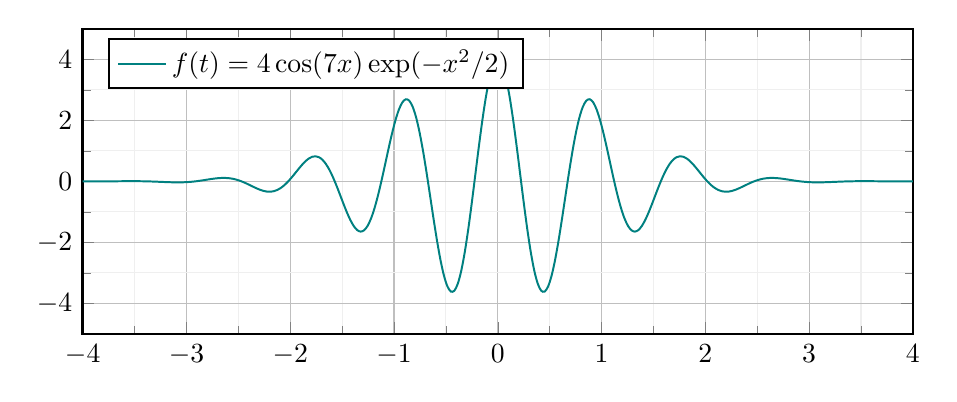
\begin{tikzpicture}
		\begin{axis}[
			grid = both,
			legend pos = north west,
			minor tick num = 1,
			major grid style = {lightgray},
			minor grid style = {lightgray!25},
			width = \textwidth,
			height = 0.45 \textwidth,
			xmin=-4, xmax=4,
			ymin=-5, ymax=5,
			line width=0.3mm
			]
			
			\addplot[domain = -5:5,
			samples = 300,
			color = teal,
			smooth,
			line width = 0.025cm,] {4 * cos(7 * deg(x)) * e^(- (x^2) / 2)};
			
			\legend{$f(t) = 4 \cos(7x)\exp(-x^2 / 2)$};
		\end{axis}
	\end{tikzpicture}
	\caption{Построение wavelet Морле (в действительной плоскости)}
\end{figure}
\noindent В формализованном виде Wavelet преобразование имеет вид:
\begin{equation}
	\begin{split}
		f(t) & = \frac{1}{2\pi C_{\psi}} \int_{\R} \int_{\R} \frac{W_{\psi}(f_{a, b})}{a^2}\psi_{a, b}(t) \; da \; db\\
		C_{\psi} & = \int_{\R} \frac{|\hat{\phi}(\omega)|^2}{|\omega|} \; d \omega
	\end{split}
\end{equation}
Где $\hat{\phi}(\omega)$ - преобразование Фурье для выбранного в качестве основного Wavelet'а. Но при этом функция, использующаяся для разложения, должна иметь конечную энергию, то есть $C_{\psi} \in \R$, более того $\int_{-\infty}^{+\infty} \psi(x) dx$ должен быть $0$. А формула прямого перехода в пространство частоты и времени, то есть формула прямого Wavelet преобразования, имеет вид:
\begin{equation}
	W_{\psi}(f_{a, b}) = \frac{1}{\sqrt{a}}\int_{\R}f(t) \overline{\phi}\left( \frac{t - b}{a} \right) \; dt
\end{equation}
Где $b$ - параметр, отвечающий за сдвиг функции wavelet по сигналу, параметр $a$ - коэффициент сжатия/растяжения wavelet, а $\overline{\phi}$ - комплексное сопряжение.

Интересно, что отличия от преобразования Фурье минимальны, так как в преобразовании Wavelet просто взяты иные базисные функции, что сохраняет саму структуру действий при проведении подобного анализа. Поэтому все основные свойства, характерные для преобразования Фурье, остаются верными. Более подробно об этом в \cite{brunton2022data}. Графики, которые получаются после проведения данного анализа называются scalograms, что на русском скейлограммы. Далее приводим пример применения Wavelet анализа к показателям Apple.

